% 1958 年不明卷（可能是某省与云南试题混合）第 4 题：四面体 ABCD（A 顶部、D 左、B 右、C 底部）被一平面所截，截口 HEFG 为平行四边形（H 在 AD 上、E 在 AC 上、F 在 CB 上、G 在 DB 上）；DB 为背面棱，虚线；截面靠背面的两边 FG、GH 亦随之绘为虚线（按源卷布局，坐标手算）
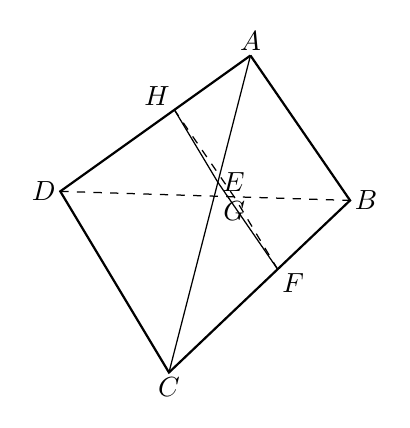
\begin{tikzpicture}[scale=1.15, line width=0.45pt,
  every node/.style={inner sep=1.5pt}]
  \coordinate (A) at (0.5,2.0);
  \coordinate (D) at (-1.6,0.5);
  \coordinate (B) at (1.6,0.4);
  \coordinate (C) at (-0.4,-1.5);
  \coordinate (H) at (-0.34,1.4);
  \coordinate (E) at (0.14,0.6);
  \coordinate (G) at (0.32,0.44);
  \coordinate (F) at (0.8,-0.36);
  \draw[line width=0.8pt] (A) -- (D) -- (C) -- (B) -- (A);
  \draw (A) -- (C);
  \draw[dashed] (D) -- (B);
  \draw (H) -- (E) -- (F);
  \draw[dashed] (F) -- (G) -- (H);
  \node[anchor=south] at (A) {$A$};
  \node[anchor=east] at (D) {$D$};
  \node[anchor=west] at (B) {$B$};
  \node[anchor=north] at (C) {$C$};
  \node[anchor=south east] at (H) {$H$};
  \node[anchor=west] at (E) {$E$};
  \node[anchor=north] at (G) {$G$};
  \node[anchor=north west] at (F) {$F$};
\end{tikzpicture}
